%
% intro.tex -- Einleitung zum Thema
%
% !TEX root = ../../buch.tex
% !TEX encoding = UTF-8
%
\section{Einleitung}

\begin{figure}
\centering
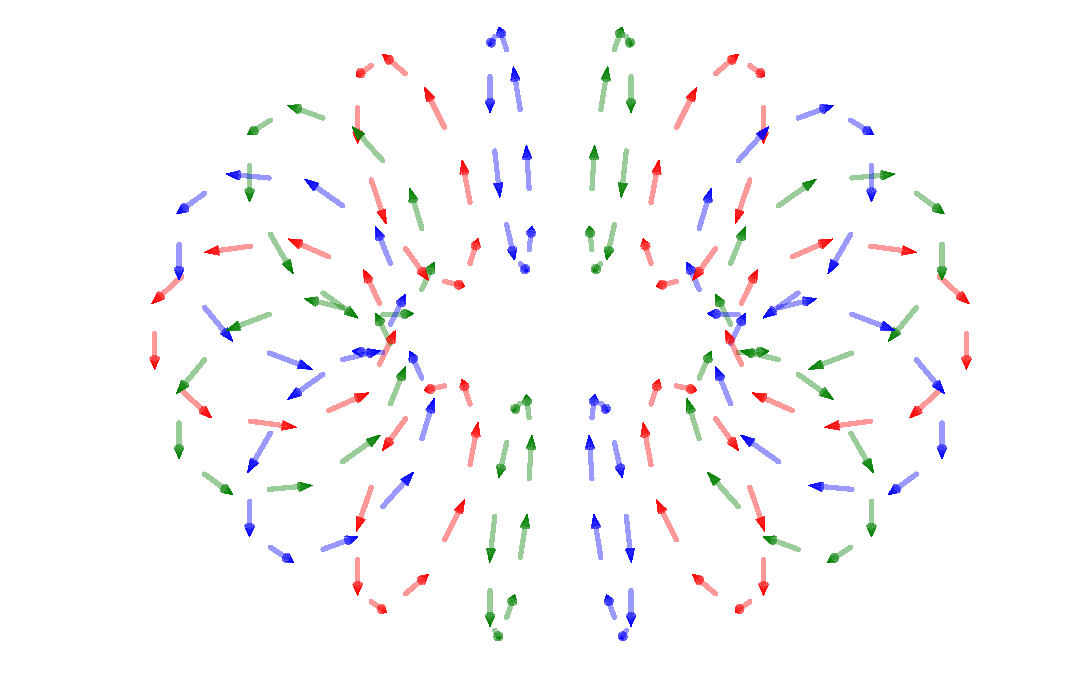
\includegraphics[width=1\textwidth]{papers/wirbelringe/fig/wirbelring_RGB.pdf}
\caption{Typischer idealer Wirbelring.
Dargestellt durch momentane Bewegungsvektoren unterschiedlicher Teilchen in regelmässigem Abstand.
Zur besseren Übersicht sind Teilchen eines Wirbels mit derselben Farbe markiert.
Unterschiedliche, benachbarte Wirbel haben unterschiedliche Farben.
Die Wirbellinie ist als schwarze, gestrichelte Linie eingezeichnet.\label{Wirbelringe:fig:generell}}
\end{figure}

ToDo

\section*{Disclaimer}

In diesem Paper werden, wo nicht anders angegeben nur ideale Fluide betrachtet.

\begin{displayquote}
    The theory of inviscid fluids is the study of «dry water».

    - John von Neumann\cite{Wirbelringe:feynman1964lectures}
\end{displayquote}

\subsection{Wirbel}

\begin{figure}
\centering
\begin{tikzpicture}
\clip (-6.3,-2.7) rectangle (6.3,2.7);
\node at (-0.07,-0.07) {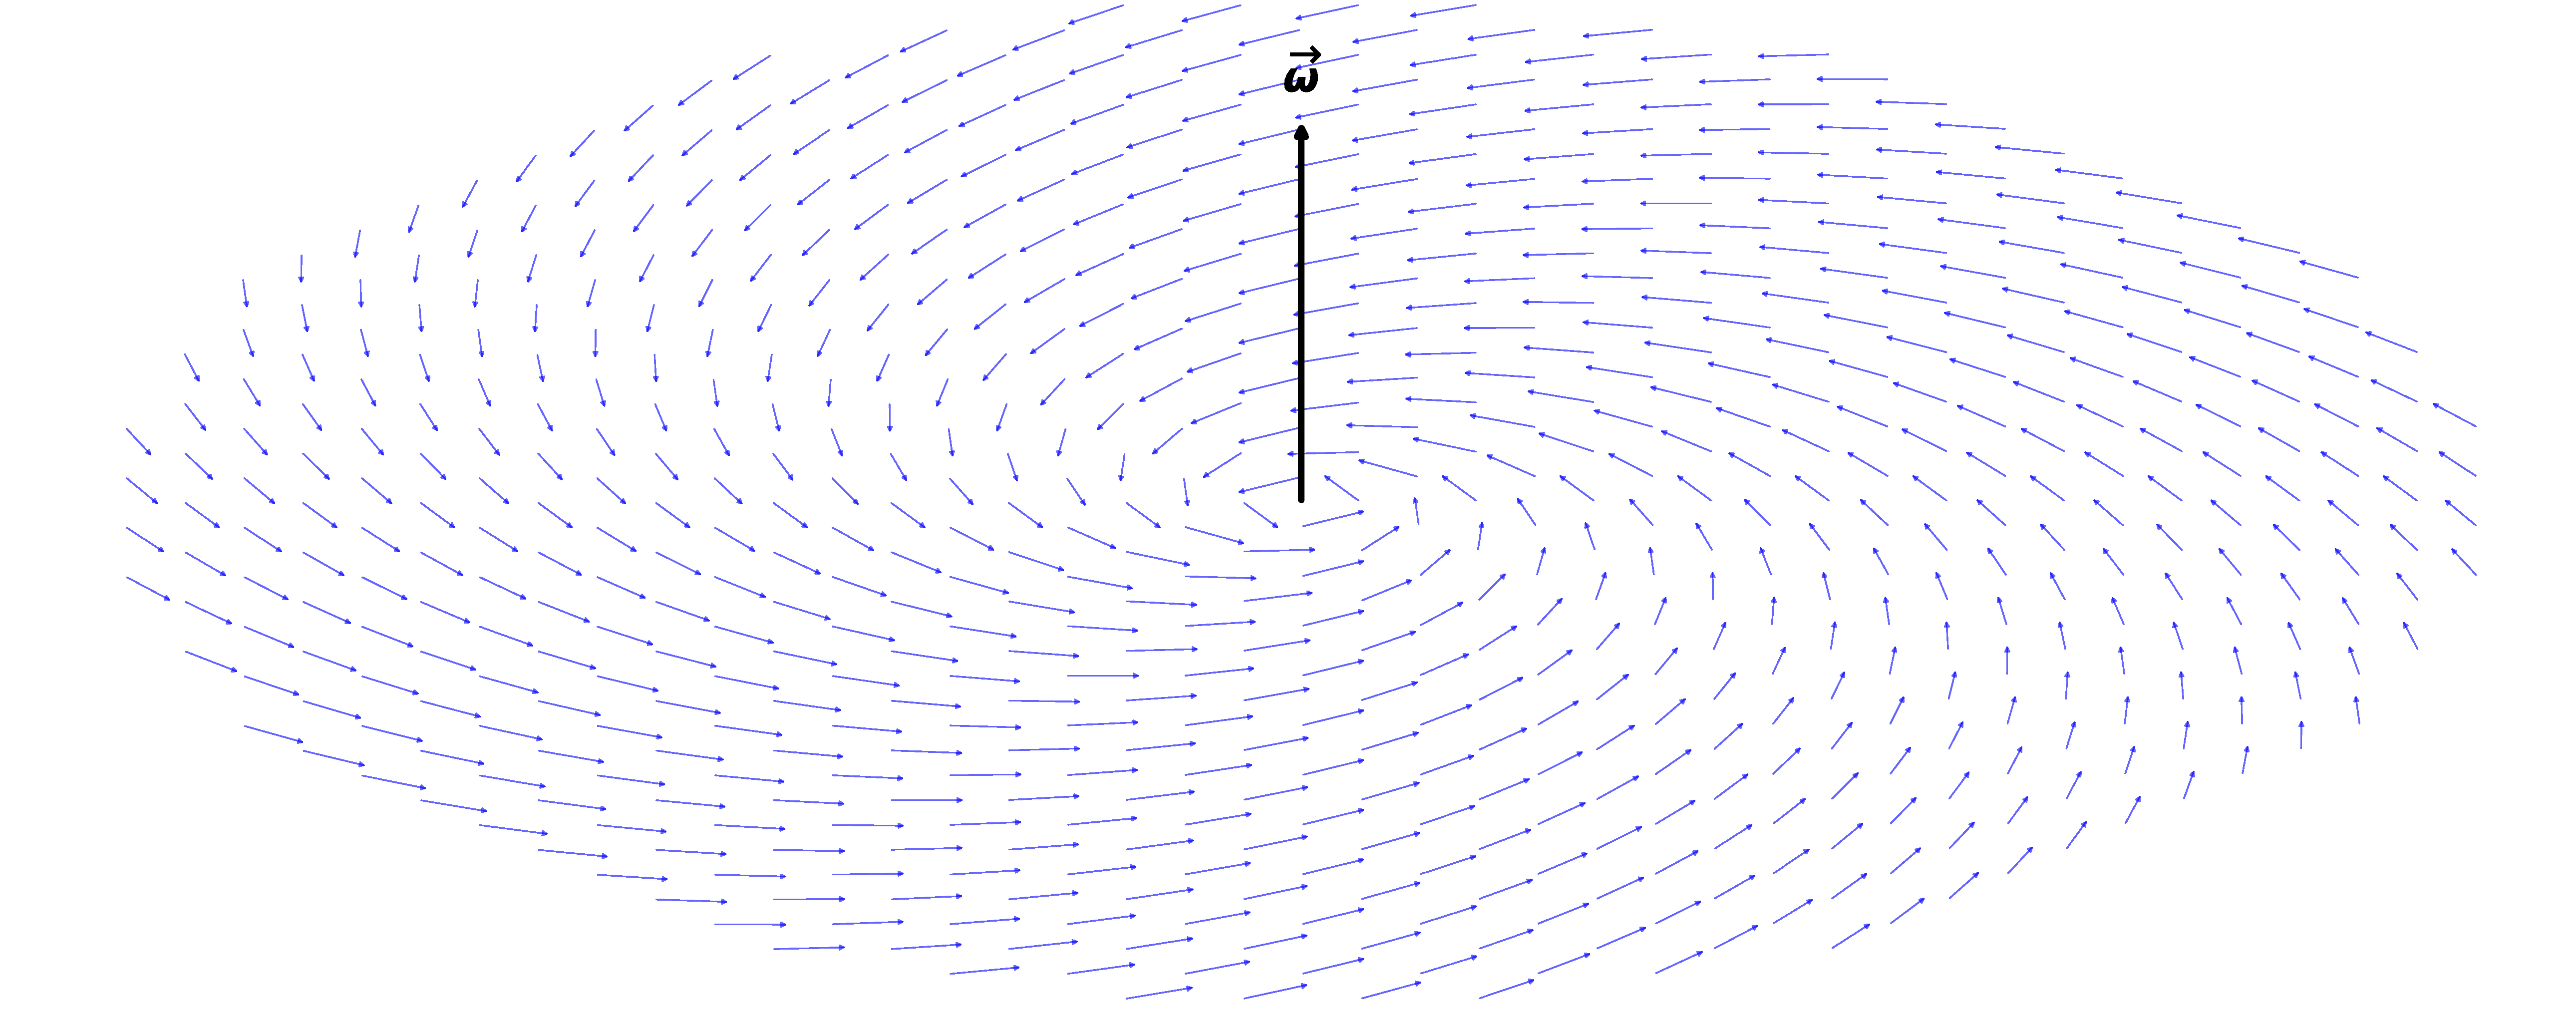
\includegraphics[width=1.08\textwidth]{papers/wirbelringe/fig/flacher_wirbel.pdf}};
%\draw[color=red] (-6.3,-2.7) rectangle (6.3,2.7);
\end{tikzpicture}
\caption{Darstellung eines 2-dimensionalen Wirbels mit Wirbelvektor
\(\vec{\omega}\).
\label{Wirbelringe:fig:flacher_wirbel}}
\end{figure}


Für die Betrachtung von Wirbelringen müssen wir zunächst einzelne Wirbel betrachten. 
In Abbildung \ref{buch:papers:Wirbelringe:fig:flacher_wirbel} ist solch ein Wirbel abgebildet. 
Für Wirbel ist die Identität
\[
\operatorname{div} \left( \operatorname{rot} \left( \vec{A} \right) \right) 
= 
0
\]
für die Stabilität eines Wirbels sehr wichtig. 
Das geht natürlich nur, wenn \(\vec{A}\) 2-mal stetig differenzierbar ist. 
Ist das der Fall kann man das ganze kurz beweisen:

\begin{gather*}
\operatorname{div} \left( \operatorname{rot} \left( \vec{A} \right) \right) 
= 0\\
\operatorname{div}      
    \begin{pmatrix} 
        \frac{\partial A_z}{\partial y} - \frac{\partial A_y}{\partial z} \\ 
        \frac{\partial A_x}{\partial z} - \frac{\partial A_z}{\partial x} \\ 
        \frac{\partial A_y}{\partial x} - \frac{\partial A_x}{\partial y} \\ 
    \end{pmatrix} 
= 0\\
\frac{\partial^2 A_z}{\partial x \partial y} - \frac{\partial^2 A_y}{\partial x \partial z} + 
\frac{\partial^2 A_x}{\partial y \partial z} - \frac{\partial^2 A_z}{\partial y \partial x} +
\frac{\partial^2 A_y}{\partial z \partial x} - \frac{\partial^2 A_x}{\partial z \partial y}
= 0\\
\frac{\partial^2 A_z}{\partial x \partial y} - \frac{\partial^2 A_z}{\partial y \partial x} + 
\frac{\partial^2 A_x}{\partial y \partial z} - \frac{\partial^2 A_x}{\partial z \partial y} +
\frac{\partial^2 A_y}{\partial z \partial x} - \frac{\partial^2 A_y}{\partial x \partial z}
= 0 \quad \text{(Satz von Schwarz)}\\
\overbrace{\frac{\partial^2 A_z}{\partial x \partial y} - \frac{\partial^2 A_z}{\partial x \partial y}}^0 + 
\overbrace{\frac{\partial^2 A_x}{\partial y \partial z} - \frac{\partial^2 A_x}{\partial y \partial z}}^0 +
\overbrace{\frac{\partial^2 A_y}{\partial x \partial z} - \frac{\partial^2 A_y}{\partial x \partial z}}^0
= 0 
\end{gather*}

Die Interpretation ist für unseren Anwendungsfall wichtiger. 
In einem reinen Quellenfeld bleiben die Teilchen erhalten. 
Das bedeutet das sie, solange nicht anders beeinflusst werden, immer weiter rotieren. 
Aus diesem Grund sind Wirbel sehr Stabil.


\subsection{Wirbel vs Wirbelring}

Werden nun viele Wirbel aneinander gereiht, entsteht ein sogenannter Wirbelfaden (Siehe Abbildung \ref{paper:Wirbelringe:Wirbelfaden}).
Dieser alleine bewegt sich allerdings noch nicht. 
Damit das passiert muss der Freie Wirbelfaden gekrümmt und zu einem Ring geschlossen werden. 
Jetzt ist es ein Wirbelring.
